\chapter{Introduzione}
\label{ch:introduzione}
Internet, è una piattaforma globale che permette a oggetti di tutti i giorni di coordinarsi e comunicare tra loro. È in quest'ottica che nasce 
Internet of Things, (IoT, Internet delle cose in italiano), la quale indica un trend attuale che prevede la connessione a Internet di ogni tipologia di oggetto fisico, 
anche alcune finora impensabili.

Oggigiorno è possibile collegare qualsiasi cosa, dagli oggetti familiari, come frigoriferi e lampadine, a risorse aziendali quali 
le etichette di spedizioni e i dispositivi medici, fino ai dispositivi indossabili, ai dispositivi intelligenti e alle città smart, la cui esistenza è esclusivamente 
dovuta all'IoT.

I primi concetti alla base dell’IoT sono stati abbozzati nel 1982, quando alcuni ricercatori della Carnegie Mellon University hanno applicato sensori
e la connessione in rete a un distributore di bibite dell’Ateneo per conoscernene lo stato di funzionamento. 

Il termine ``Internet of Things" fu coniato, però, per la prima volta solo nel 1999 dall'imprenditore inglese Kevin Ashton per descrivere la connessione di oggetti del 
mondo fisico ad Internet, Kevin mostra i limiti di una tecnologia basata solo sulle idee, su dati generati dagli utenti e vede, invece, le prospettive che possono 
offrire gli oggetti di tutti i giorni connessi in rete, in grado di fornirci informazioni sul loro stato, permettendoci quindi di sapere quando uno di essi necessita 
di essere riparato o sostituito.

A oggi, come si può notare dal grafico in Figura~\ref{IOTgraph}, il numero di dispositivi connessi è in continua crescita, anche perchè i campi di applicazione sono numerosi, 
questo grazie alle enormi potenzialità che oggetti di tutti i giorni possano offrirci se connessi a Internet e/o interconnessi tra di loro equipaggiandoli 
all'occorenza con svariati sensori.
I campi in cui Internet of Things si è affermato maggiormente sono i seguenti:
\begin{itemize}
    \item Domotica
    \item Smart City
    \item Industria
    \item Agricoltura
    \item Logistica e trasporto
\end{itemize}
\begin{figure}[htb]
    \centering
    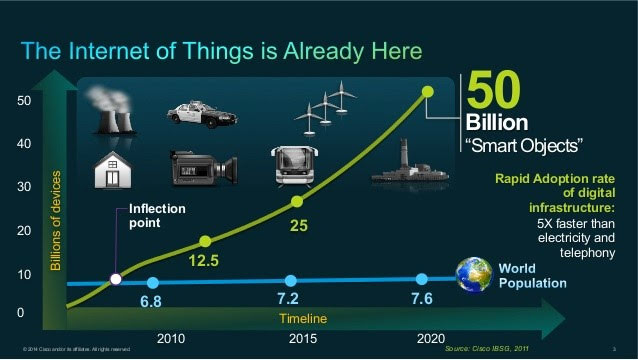
\includegraphics[width=0.7\textwidth]{images/IoT-graph.png}
    \caption{Grafico crescita del numero di dispositivi connessi.}
    \label{IOTgraph}
\end{figure}
Un report di Business Insider Intelligence~\cite{insiderIntelligence} afferma che, nei prossimi cinque anni arriveremo a 40 miliardi di dispositivi IoT mentre
i governi , entro il 2023, investiranno circa 900 miliardi di dollari per lo sviluppo di smart city, smart utility e sistemi di telecamere connesse. 
Negli Usa i dispositivi domestici smart supereranno il miliardo entro il 2023, con un consumo stimato di circa 725 dollari per famiglia, per un totale di oltre 
90 miliardi di dollari in spese per soluzioni IoT. Numeri in crescita anche nel settore industriale, infatti le imprese continueranno a investire miliardi nel settore , 
in particolare , entro il 2023 la spesa annuale per la produzione di soluzioni IoT raggiungerà circa 450 miliardi di dollari, mentre la base installata totale di sistemi 
robotici industriali raggiungerà i 6 milioni in tutto il mondo.

Stando ai dati sopra riportati ci sarà un forte aumento dei dispositivi connessi e conseguentemente aumenteranno anche i dati prodotti. Purtroppo, a fronte di uno 
scenario che fa crescere le opportunità di business e di ricchezza aumenteranno anche le minacce che porteranno ad un problema sia per quanto riguarda la sicurezza 
in generale che per quella associata alla protezione dei dati personali.

La società di ricerca Gartner nello studio “Worldwide IoT security spending forecast 2018-2021 per segment” porta l’attenzione sui rischi e sulle vulnerabilità 
collegate alla diffusione dell’Internet delle cose, pericolo alimentato peraltro anche dalla semplicità delle componenti informatiche integrate in elettrodomestici (se
si parla delle smart Home) e altri oggetti abilitati dall’IoT, unitamente a difetti della gestione e dell’aggiornamento, infatti come riportato 
nell'articolo~\cite{articoloSicurezza} negli ultimi tre anni un’azienda su 5 ha subito almeno un attacco ai propri ambienti Internet of Things. 

Il rischio per la sicurezza non riguarderà più solo server, computer o device mobili in dotazione al personale, ma tutti gli oggetti intelligenti 
che raccolgono dati e aiutano a governare edifici, produzioni, e apparti dai quali dipendono servizi di mobilità, rischio divenuto realtà quando ad esempio 
una variante del malware Mirai, chiamata OMG ha colpito gli endpoint IoT consentendo a malintenzionati di portare avanti attacchi Denial of Service su 
larga scala (dove i dispositivi infettati generavano traffico fittizio per saturare siti e servizi).

Nei prossimi anni le piattaforme IoT rischiano quindi di essere sempre più frequentemente soggette ad attacchi informatici via via più sofisticati. 
Le modalità di difesa possono essere: 
\begin{itemize}
    \item Scegliere prodotti IoT affidabili dotati di protezioni specifiche.
    \item Curare le configurazioni dei dispositivi usando credenziali di autenticazione (password) più sicure
    e assicurando l’applicazione delle patch, aggiornando sistemi operativi, driver e programmi di gestione.
    \item Cifrare i dati trasmessi da un punto all'altro implementando uno dei tanti protocolli crittografici.
    \item Analizzare i possibili attacchi in quanto , a volte , vengono attuati attacchi pensati specificamente per compromettere determinate aziende o determinate 
    attività. E’ quindi necessario progettare e applicare forme di protezione personalizzate e specificatamente indirizzate a proteggere aziende anche da precise minacce.
    \item A livello di rete si può invece limitare al minimo indispensabile la banda e altri servizi accessibili ai dispositivi IoT, quindi rilevare e segnalare 
    agli amministratori le anomalie riconducibili a possibili infezioni.
\end{itemize}